\documentclass[12pt]{article}
\usepackage{graphicx}
\usepackage{amsmath}
\usepackage{amssymb}
\usepackage{color}
\usepackage{braket}
\usepackage[margin=1in]{geometry}
\usepackage{mathtools}
\usepackage{tikz}

\allowdisplaybreaks
\numberwithin{equation}{section}

\interfootnotelinepenalty=10000

\usepackage{calligra}
\usepackage{hyperref}
\hypersetup{colorlinks=true, linkcolor=blue}

\DeclareMathAlphabet{\mathcalligra}{T1}{calligra}{m}{n}
\DeclareFontShape{T1}{calligra}{m}{n}{<->s*[2.2]callig15}{}
\newcommand{\scriptr}{\mathcalligra{r}\,}
\newcommand{\boldscriptr}{\pmb{\mathcalligra{r}}\,}

\newcommand{\Lagr}{\mathcal{L}}
\newcommand{\Hami}{\mathcal{H}}
\newcommand{\reals}{\rm I\!R}
\newcommand{\order}{\mathcal{O}}
\newcommand{\bx}{\mathbf{x}}
\newcommand{\bp}{\mathbf{p}}
\newcommand{\bq}{\mathbf{q}}
\newcommand{\redtext}[1]{\textcolor{red}{#1}}
\newcommand{\pvec}[1]{\vec{#1}\mkern2mu\vphantom{#1}}


\begin{document}
	\title{Numerical Relativity Project \#1}
	\author{Alex Pandya}
	\date{March 27th, 2018}
	\maketitle

\section{Problem 1a)}
In this problem we are given the static, spherically symmetric, vacuum metric (Schwarzschild metric)
\begin{equation} \label{eq:metric}
ds^2 = (-\alpha^2 + a^2 \beta^2) dt^2 + 2 a^2 \beta dt dr + a^2 dr^2 + r^2 (d\theta^2 + \sin^2 \theta d\phi^2),
\end{equation}
and we are asked to compute the characteristics (null geodesics) of the given metric.  We are given that we are working in spherical symmetry, so we want radial null geodesics; thus we want $dr/dt$.  Starting with the metric and zeroing out $ds$, $d\theta$ and $d\phi$, we get:
\begin{equation}
\begin{aligned}
0 &= (-\alpha^2 + a^2 \beta^2) dt^2 + 2 a^2 \beta dt dr + a^2 dr^2 \\
0 &= (-\alpha^2 + a^2 \beta^2) + 2 a^2 \beta \frac{dr}{dt} + a^2 \frac{dr^2}{dt^2}, \\
\end{aligned}
\end{equation}
which is quadratic in $dr/dt$.  Solving via the quadratic formula, we get
\begin{equation} \label{eq:c_plus_eqn}
\begin{aligned}
\Big(\frac{dr}{dt}\Big)_\pm &= \frac{-2 a^2 \beta \pm \sqrt{4 a^4 \beta^2 - 4 a^2 (-\alpha^2 + a^2 \beta^2)}}{2 a^2} \\
&= - \beta \pm \sqrt{\beta^2 + \frac{\alpha^2}{a^2} - \beta^2} \\
&= - \beta \pm \frac{\alpha}{a}, \\
\end{aligned}
\end{equation}
as we were asked to show.

\section{Problem 1b)}
We are now asked to write down the equation of motion for a massless Klein-Gordon field in a spacetime described by the above metric (equation \ref{eq:metric}):
\begin{equation} \label{eq:massless_KGE}
\nabla_a \nabla^a \phi = 0.
\end{equation}

\subsection{Christoffel Symbol Identity}

In order to evaluate this, we will need an identity.  Since we have the contraction of two covariant derivatives, above, we need to evaluate $\nabla^a (\nabla_a \phi)$, which is a covariant divergence.  Carroll gives a formula for the covariant divergence, which I will derive here.

Starting from the definition of the covariant derivative, we find
\begin{equation}
\nabla_\mu V^\mu = \partial_\mu V^\mu + \Gamma^\mu_{\mu \lambda} V^\lambda,
\end{equation}
and we aim to simplify the Christoffel symbol on the right-hand side.  Applying the definition of the Christoffel symbol, we find:
\begin{equation} \label{eq:divergence_christoffel_symbol}
\begin{aligned}
\Gamma^{\mu}_{\mu \lambda} &= \frac{1}{2} g^{\mu \rho} (\partial_\mu g_{\lambda \rho} + \partial_{\lambda} g_{\rho \mu} - \partial_\rho g_{\mu \lambda}) \\
&= \frac{1}{2} g^{\mu \rho} \partial_\mu g_{\lambda \rho} + \frac{1}{2} g^{\mu \rho} \partial_{\lambda} g_{\rho \mu} - \frac{1}{2} g^{\mu \rho} \partial_\rho g_{\mu \lambda} \\
&= \frac{1}{2} g^{\mu \rho} \partial_\mu g_{\lambda \rho} + \frac{1}{2} g^{\mu \rho} \partial_{\lambda} g_{\rho \mu} - \frac{1}{2} g^{\rho \mu} \partial_\rho g_{\lambda \mu} \\
&= \frac{1}{2} g^{\nu \sigma} \partial_\nu g_{\lambda \sigma} + \frac{1}{2} g^{\mu \rho} \partial_{\lambda} g_{\rho \mu} - \frac{1}{2} g^{\nu \sigma} \partial_\nu g_{\lambda \sigma} \\
&= \frac{1}{2} g^{\mu \rho} \partial_{\lambda} g_{\rho \mu}, \\
\end{aligned}
\end{equation}
where in the third line we have used the symmetry of the metric twice on the third term, and in the fourth line we have relabeled dummy indices to make the cancellation (done in the fifth line) more obvious.  We now make use of Jacobi's formula\footnote{See the Wikipedia article on Jacobi's formula.}
\begin{equation} \label{eq:jacobi_formula}
\partial_\lambda \mathrm{Det}[\textbf{A}] = \mathrm{Tr}[\mathrm{adj}(\textbf{A}) \partial_\lambda \textbf{A}],
\end{equation}
where the \textit{adjugate} of the matrix $A$ is defined such that
\begin{equation}
\textbf{A} ~\mathrm{adj}(\textbf{A}) = \mathrm{Det}[\textbf{A}] \textbf{I},
\end{equation}
where $\textbf{I}$ is the identity matrix.  We also need Cramer's rule\footnote{See the Wikipedia article for Cramer's rule -- specifically the section ``Finding inverse matrix."} for the inverse of a matrix:
\begin{equation}
\textbf{A}^{-1} = \frac{1}{\mathrm{Det}[\textbf{A}]} \mathrm{adj}(\textbf{A}).
\end{equation}

In the context of GR, we are interested in utilizing the metric and the inverse metric.  Let's now consider
\begin{equation*}
\begin{aligned}
\frac{1}{\sqrt{\mathrm{Det}[\textbf{g}]}} \partial_\lambda \sqrt{\mathrm{Det}[\textbf{g}]} &= \frac{1}{\sqrt{\mathrm{Det}[\textbf{g}]}} \Big(\frac{1}{2} \frac{1}{\sqrt{\mathrm{Det}[\textbf{g}]}} \partial_\lambda \mathrm{Det}[\textbf{g}] \Big) \\
&= \frac{1}{2} \frac{1}{\mathrm{Det}[\textbf{g}]} \partial_\lambda \mathrm{Det}[\textbf{g}] \\
&= \frac{1}{2} \frac{1}{\mathrm{Det}[\textbf{g}]} \mathrm{Tr}[\mathrm{adj}(\textbf{g}) \partial_\lambda \textbf{g}] \\
&= \frac{1}{2} \frac{1}{\mathrm{Det}[\textbf{g}]} \mathrm{Tr}[ \mathrm{Det}[\textbf{g}] \textbf{g}^{-1} \partial_\lambda \textbf{g}] \\
&= \frac{1}{2} \mathrm{Tr}[ \textbf{g}^{-1} \partial_\lambda \textbf{g}] \\
&= \frac{1}{2} g^{\mu \rho} \partial_{\lambda} g_{\rho \mu},
\end{aligned}
\end{equation*}
which is equal to the final line of equation \ref{eq:divergence_christoffel_symbol}.  Thus we have the identity
\begin{equation}
\Gamma^\mu_{\mu \lambda} = \frac{1}{\sqrt{|g|}} \partial_\lambda \sqrt{|g|}.
\end{equation}

\subsection{Covariant Divergence Identity}

Using this identity, we have that
\begin{equation} \label{eq:divergence_identity}
\begin{aligned}
\nabla_\mu V^\mu &= \partial_\mu V^\mu + V^\mu \frac{1}{\sqrt{|g|}} \partial_\lambda \sqrt{|g|} \\
&= \frac{1}{\sqrt{|g|}} \partial_\mu (V^\mu \sqrt{|g|}).
\end{aligned}
\end{equation}

\subsection{Applying the Identities}
Applying the divergence identity (equation \ref{eq:divergence_identity}) to the massless Klein-Gordon equation (equation \ref{eq:massless_KGE}) we find
\begin{equation} \label{eq:KGE_hint_form}
\begin{aligned}
\nabla_a \nabla^a \phi &= \nabla_\mu (g^{\mu \nu}\partial_\nu \phi) \\
&= \frac{1}{\sqrt{|g|}} \partial_\mu (g^{\mu \nu} \sqrt{|g|} \partial_\nu \phi),
\end{aligned}
\end{equation}
as we are asked to show in the \textbf{Hint} section of the problem.  We now  need to compute the inverse metric $g^{\mu \nu}$.  We may do so using the condition
\begin{equation}
g_{a b} g^{b c} = \delta_a^c,
\end{equation}
which implies the equations
\begin{equation}
\begin{aligned}
g^{rr} &= g^{tt} \Big(-\frac{\alpha^2}{a^2} + \beta^2\Big) \\
(-\alpha^2 + a^2 \beta^2) g^{tr} &= -a^2 \beta g^{rr} \\
g^{rt} &= -\beta g^{tt} \\
a^2 \beta g^{tr} + a^2 g^{rr} &= 1 \\
g^{\theta \theta} &= r^{-2} \\
g^{\phi \phi} &= r^{-2} \sin^{-2} \theta,
\end{aligned}
\end{equation}
which may be used along with the symmetry of the metric (and inverse metric) to yield
\begin{equation} \label{eq:inverse_metric}
g^{\mu \nu} =
\begin{pmatrix}
-\alpha^{-2} & \beta \alpha^{-2} & 0 & 0 \\
\beta \alpha^{-2} & a^{-2} - \beta^{2} \alpha^{-2} & 0 & 0 \\
0 & 0 & r^{-2} & 0 \\
0 & 0 & 0 & r^{-2} \sin^{-2} \theta
\end{pmatrix}.
\end{equation}

We can now expand out the Klein-Gordon equation (equation \ref{eq:KGE_hint_form}):
\begin{equation} \label{eq:KGE_expanded}
\begin{aligned}
\nabla_a \nabla^a \phi &= \frac{1}{\sqrt{|g|}} \partial_\mu (g^{\mu \nu} \sqrt{|g|} \partial_\nu \phi) \\
&= \frac{1}{a \alpha r^2 \sin \theta} \partial_\mu (g^{\mu \nu} a \alpha r^2 \sin \theta \partial_\nu \phi) \\
&= \frac{1}{r^2 \sin \theta} \partial_\mu (g^{\mu \nu} r^2 \sin \theta \partial_\nu \phi), \\
\end{aligned}
\end{equation}
where we have used the fact that $|g| = a^2 \alpha^2 r^4 \sin^2 \theta$.  We may now expand out the Einstein-notation sum to get
\begin{equation*}
\begin{aligned}
&= \frac{1}{r^2 \sin \theta} \partial_t (g^{t \nu} r^2 \sin \theta \partial_\nu \phi) + \frac{1}{r^2 \sin \theta} \partial_r (g^{r \nu} r^2 \sin \theta \partial_\nu \phi) \\
&+ \frac{1}{r^2 \sin \theta} \partial_\theta (g^{\theta \nu} r^2 \sin \theta \partial_\nu \phi) + \frac{1}{r^2 \sin \theta} \partial_\varphi (g^{\varphi \nu} r^2 \sin \theta \partial_\nu \phi)\\
&= \frac{1}{r^2 \sin \theta} \partial_t (g^{t t} r^2 \sin \theta \partial_t \phi) + \frac{1}{r^2 \sin \theta} \partial_t (g^{t r} r^2 \sin \theta \partial_r \phi) + \frac{1}{r^2 \sin \theta} \partial_r (g^{r t} r^2 \sin \theta \partial_t \phi) \\
&+ \frac{1}{r^2 \sin \theta} \partial_r (g^{r r} r^2 \sin \theta \partial_r \phi) + \frac{1}{r^2 \sin \theta} \partial_\theta (g^{\theta \theta} r^2 \sin \theta \partial_\theta \phi) + \frac{1}{r^2 \sin \theta} \partial_\varphi (g^{\varphi \varphi} r^2 \sin \theta \partial_\varphi \phi), \\
\end{aligned}
\end{equation*}
we now note that everything in our problem is spherically symmetric, so the $\partial_\theta \phi$ and $\partial_\varphi \phi$ terms must be zero.  Thus
\begin{equation*}
\begin{aligned}
&= \frac{1}{r^2 \sin \theta} \partial_t (g^{t t} r^2 \sin \theta \partial_t \phi) + \frac{1}{r^2 \sin \theta} \partial_t (g^{t r} r^2 \sin \theta \partial_r \phi) \\
&+ \frac{1}{r^2 \sin \theta} \partial_r (g^{r t} r^2 \sin \theta \partial_t \phi) + \frac{1}{r^2 \sin \theta} \partial_r (g^{r r} r^2 \sin \theta \partial_r \phi)\\
&= \frac{1}{r^2 \sin \theta} \partial_t ( (-\alpha^{-2}) r^2 \sin \theta \partial_t \phi) + \frac{1}{r^2 \sin \theta} \partial_t ( (\beta \alpha^{-2}) r^2 \sin \theta \partial_r \phi) \\
&+ \frac{1}{r^2 \sin \theta} \partial_r ( (\beta \alpha^{-2}) r^2 \sin \theta \partial_t \phi) + \frac{1}{r^2 \sin \theta} \partial_r ( (a^{-2} - \beta^2 \alpha^{-2}) r^2 \sin \theta \partial_r \phi)\\
&= -\alpha^{-2} \partial_t \partial_t \phi + \beta \alpha^{-2} \partial_t  \partial_r \phi + \frac{\beta \alpha^{-2}}{r^2} \partial_r ( r^2 \partial_t \phi) + \frac{(a^{-2} - \beta^2 \alpha^{-2})}{r^2} \partial_r (r^2 \partial_r \phi)\\
&= -\alpha^{-2} \partial_t \partial_t \phi + \beta \alpha^{-2} \partial_t  \partial_r \phi \\
&+ \frac{\beta \alpha^{-2}}{r^2} (2 r \partial_t \phi + r^2 \partial_r \partial_t \phi) + \frac{(a^{-2} - \beta^2 \alpha^{-2})}{r^2} (2 r \partial_r \phi + r^2 \partial_r \partial_r \phi)\\
&= -\alpha^{-2} \partial_t \partial_t \phi + \beta \alpha^{-2} \partial_t  \partial_r \phi + \frac{\beta \alpha^{-2}}{r^2} 2 r \partial_t \phi + \frac{\beta \alpha^{-2}}{r^2} r^2 \partial_r \partial_t \phi \\
&+ \frac{2a^{-2}}{r} \partial_r \phi - \frac{2\beta^2 \alpha^{-2}}{r} \partial_r \phi + a^{-2} \partial_r \partial_r \phi - \beta^2 \alpha^{-2} \partial_r \partial_r \phi \\
&= -\alpha^{-2} \partial_t \partial_t \phi + (\beta \alpha^{-2} \partial_t  \partial_r \phi - \beta^2 \alpha^{-2} \partial_r \partial_r \phi) + \Big( \frac{2 \beta \alpha^{-2}}{r} \partial_t \phi - \frac{2\beta^2 \alpha^{-2}}{r} \partial_r \phi \Big) \\
&+ \frac{2a^{-2}}{r} \partial_r \phi + a^{-2} \partial_r \partial_r \phi + \beta \alpha^{-2} \partial_r \partial_t \phi \\
&= - \alpha^{-2} \partial_t (\partial_t \phi - \beta \partial_r \phi) + \beta \alpha^{-2} \partial_r (\partial_t  \phi - \beta \partial_r \phi) \\
&+ \frac{2\beta \alpha^{-2}}{r} (\partial_t \phi - \beta \partial_r \phi ) + \frac{2a^{-2}}{r} \partial_r \phi + a^{-2} \partial_r \partial_r \phi;\\
\end{aligned}
\end{equation*}
we now make the definitions
\begin{align}
\Phi(r, t) &= \partial_r \phi \label{eq:Phi_defn}\\
\Pi(r, t)  &= \frac{a}{\alpha} (\partial_t \phi - \beta \partial_r \phi), \label{eq:Pi_defn}
\end{align}
so the Klein-Gordon equation becomes
\begin{equation*}
\begin{aligned}
0 &= - \alpha^{-1} a^{-1} \partial_t \Pi + \beta \alpha^{-1} a^{-1} \partial_r \Pi + \frac{2\beta \alpha^{-1} a^{-1}}{r} \Pi + \frac{2a^{-2}}{r} \Phi + a^{-2} \partial_r \Phi \\
\partial_t \Pi &= \beta \partial_r \Pi + \frac{2\beta}{r} \Pi + \frac{2 \alpha}{a r} \Phi + \frac{\alpha}{a} \partial_r \Phi \\
\partial_t \Pi &= \beta \partial_r \Pi + \frac{\alpha}{a} \partial_r \Phi + \frac{2}{r} \beta \Pi + \frac{2}{r} \frac{\alpha}{a} \Phi \\
\partial_t \Pi &= \frac{1}{r^2} \partial_r \Big( r^2 \Big( \beta \Pi + \frac{\alpha}{a} \Phi \Big) \Big).
\end{aligned}
\end{equation*}

Taking a derivative with respect to $r$ of equation \ref{eq:Pi_defn} yields the other equation of motion
\begin{equation*}
\begin{aligned}
\partial_r \Pi &= \frac{a}{\alpha} (\partial_t \partial_r \phi - \beta \partial_r \partial_r \phi) \\
\partial_r \Pi &= \frac{a}{\alpha} \partial_t \Phi - \beta \frac{a}{\alpha} \partial_r \Phi \\
\partial_t \Phi &= \partial_r \Big( \beta \Phi + \frac{\alpha}{a} \Pi \Big), \\
\end{aligned}
\end{equation*}
so in summary we get equations of motion
\begin{align}
\partial_t \Phi &= \partial_r \Big( \beta \Phi + \frac{\alpha}{a} \Pi \Big) \label{eq:Phi_EOM} \\
\partial_t \Pi &= \frac{1}{r^2} \partial_r \Big( r^2 \Big( \beta \Pi + \frac{\alpha}{a} \Phi \Big) \Big). \label{eq:Pi_EOM}
\end{align}

\section{Problem 1c)}
We are now asked to consider the Schwarzschild form of the metric, which is
\begin{equation}
ds^2 = - \Big( 1 - \frac{2 M}{r} \Big) dt^2 + \Big(1 - \frac{2 M}{r} \Big)^{-1} dr^2 + r^2 d\Omega^2
\end{equation}
and to define the ``Regge-Wheeler" tortoise coordinate
\begin{equation}
r_\star \equiv r + 2 M \ln \Big( \frac{r}{2 M} - 1 \Big),
\end{equation}
and outgoing/ingoing radial coordinates
\begin{equation}
\begin{aligned}
u &= t - r_\star \\
u &= t + r_\star,
\end{aligned}
\end{equation}
and finally a new time coordinate
\begin{equation}
\tilde{t} = v - r = t + 2 M \ln \Big( \frac{r}{2 M} - 1 \Big).
\end{equation}
Using these definitions, we are asked to find the metric in terms of the coordinates $\tilde{t}, r, \Omega$.

The only major change is that we need to find $d \tilde{t}$:
\begin{equation*}
\begin{aligned}
d\tilde{t} &= dt + \frac{2 M}{r - 2 M} dr \\
d\tilde{t} - \frac{2 M}{r - 2 M} dr &= dt \\
\end{aligned}
\end{equation*}
so
\begin{equation*}
dt^2 = d\tilde{t}^2 - \frac{4 M}{r - 2 M} d\tilde{t} dr + \frac{4 M^2}{(r - 2 M)^2} dr^2
\end{equation*}
and the metric becomes
\begin{equation*}
\begin{aligned}
ds^2 &= - \Big( 1 - \frac{2 M}{r} \Big) \Big[ d\tilde{t}^2 - \frac{4 M}{r - 2 M} d\tilde{t} dr + \frac{4 M^2}{(r - 2 M)^2} dr^2 \Big] + \Big(1 - \frac{2 M}{r} \Big)^{-1} dr^2 + r^2 d\Omega^2 \\
&= - \Big( 1 - \frac{2 M}{r} \Big) d\tilde{t}^2 + \Big( 1 - \frac{2 M}{r} \Big) \frac{4 M}{r - 2 M} d\tilde{t} dr - \Big( 1 - \frac{2 M}{r} \Big) \frac{4 M^2}{(r - 2 M)^2} dr^2 \\
&+ \Big(1 - \frac{2 M}{r} \Big)^{-1} dr^2 + r^2 d\Omega^2 \\
&= - \Big( 1 - \frac{2 M}{r} \Big) d\tilde{t}^2 + \frac{4 M}{r} d\tilde{t} dr - \frac{4 M^2}{r (r - 2 M)} dr^2 + \Big(1 - \frac{2 M}{r} \Big)^{-1} dr^2 + r^2 d\Omega^2 \\
&= - \Big( 1 - \frac{2 M}{r} \Big) d\tilde{t}^2 + \frac{4 M}{r} d\tilde{t} dr + \frac{r^2 - 4 M^2}{r(r - 2M)} dr^2 + r^2 d\Omega^2 \\
&= - \Big( 1 - \frac{2 M}{r} \Big) d\tilde{t}^2 + \frac{4 M}{r} d\tilde{t} dr + \frac{(r - 2 M) (r + 2 M)}{r(r - 2M)} dr^2 + r^2 d\Omega^2, \\
\end{aligned}
\end{equation*}
so we finally get the \textit{ingoing Eddington-Finkelstein} (IEF) form of the metric:
\begin{equation} \label{eq:IEF_metric}
ds^2 = - \Big( 1 - \frac{2 M}{r} \Big) d\tilde{t}^2 + \frac{4 M}{r} d\tilde{t} dr + \Big( 1 + \frac{2 M}{r} \Big) dr^2 + r^2 d\Omega^2,
\end{equation}
which is well-behaved for $r \geq 2 M$.

\section{Problem 1d)}
We are now asked to compare the metric in IEF form (equation \ref{eq:IEF_metric}) to that in equation \ref{eq:metric} to determine the values of $a, \alpha, \beta$.  By inspection, we see that
\begin{equation}
\begin{aligned}
a^2 &= \Big(1 + \frac{2 M}{r} \Big) \\
\implies a &= \Big( \frac{r + 2 M}{r} \Big)^{1/2}
\end{aligned}
\end{equation}
and
\begin{equation}
\begin{aligned}
2 a^2 \beta &= \frac{4 M}{r} \\
\implies \beta &= \frac{2 M}{r + 2 M},
\end{aligned}
\end{equation}
and
\begin{equation}
\begin{aligned}
-\alpha^2 + a^2 \beta^2 &= - \Big( 1 - \frac{2 M}{r} \Big) \\
-\alpha^2 &= - \Big( 1 - \frac{2 M}{r} \Big) - \Big(1 + \frac{2 M}{r} \Big) \Big( \frac{2 M}{r + 2 M} \Big)^2 \\
\alpha^2 &= \frac{r - 2 M}{r} + \frac{r + 2 M}{r} \frac{4 M^2}{(r + 2 M)^2} \\
&= \frac{(r - 2 M) (r + 2 M)}{r (r + 2M)} + \frac{4 M^2}{r (r + 2 M)} \\
&= \frac{r}{r + 2M} \\
\implies \alpha &= \Big( \frac{r}{r + 2 M} \Big)^{1/2} = a^{-1}.
\end{aligned}
\end{equation}

\section{Problem 1e)}
In this problem, we are first asked to note that in the limit $r \to \infty$, the IEF metric (equation \ref{eq:IEF_metric}) approaches the Minkowski metric in spherical coordinates.  We are now asked to take this limit of the Klein-Gordon equation (equation \ref{eq:KGE_hint_form}).

Starting with equation \ref{eq:KGE_expanded} and using the Minkowski metric in spherical coordinates:
\begin{equation}
g^{\mu \nu}_{\mathrm{Minkowski}} = 
\begin{pmatrix}
-1 & 0 & 0 & 0 \\
0 & 1 & 0 & 0 \\
0 & 0 & r^{-2} & 0 \\
0 & 0 & 0 & r^{-2} \sin^{-2} \theta
\end{pmatrix},
\end{equation}
we have
\begin{equation}
\begin{aligned}
0 = \nabla_a \nabla^a \phi &= \frac{1}{r^2 \sin \theta} \partial_\mu (g^{\mu \nu} r^2 \sin \theta \partial_\nu \phi) \\
&= \frac{1}{r^2 \sin \theta} \partial_t (g^{t \nu} r^2 \sin \theta \partial_\nu \phi) + \frac{1}{r^2 \sin \theta} \partial_r (g^{r \nu} r^2 \sin \theta \partial_\nu \phi) \\
&+ \frac{1}{r^2 \sin \theta} \partial_\theta (g^{\theta \nu} r^2 \sin \theta \partial_\nu \phi) + \frac{1}{r^2 \sin \theta} \partial_\varphi (g^{\varphi \nu} r^2 \sin \theta \partial_\nu \phi) \\
&= \frac{1}{r^2 \sin \theta} \partial_t (g^{t t} r^2 \sin \theta \partial_t \phi) + \frac{1}{r^2 \sin \theta} \partial_r (g^{r r} r^2 \sin \theta \partial_r \phi) \\
&+ \frac{1}{r^2 \sin \theta} \partial_\theta (g^{\theta \theta} r^2 \sin \theta \partial_\theta \phi) + \frac{1}{r^2 \sin \theta} \partial_\varphi (g^{\varphi \varphi} r^2 \sin \theta \partial_\varphi \phi) \\
&= - \partial_t (\partial_t \phi) + \frac{1}{r^2} \partial_r (r^2 \partial_r \phi) + \frac{1}{r^2 \sin \theta} \partial_\theta (\sin \theta \partial_\theta \phi) + \frac{1}{r^2 \sin \theta} \partial_\varphi (\partial_\varphi \phi). \\
\end{aligned}
\end{equation}
We may now use the fact that the problem is spherically symmetric to assert that $\partial_\theta \phi = \partial_\varphi \phi = 0$, and we get:
\begin{equation*}
\begin{aligned}
0 &= - \partial_t (\partial_t \phi) + \frac{1}{r^2} \partial_r (r^2 \partial_r \phi) \\
\partial_{tt} \phi &= \frac{1}{r^2} (2 r \partial_r \phi + r^2 \partial_{rr} \phi) \\
\partial_{tt} \phi &= \frac{2}{r} \partial_r \phi + \partial_{rr} \phi \\
r \partial_{tt} \phi &= 2 \partial_r \phi + r \partial_{rr} \phi \\
\end{aligned}
\end{equation*}
which may be written
\begin{equation}
\partial_{tt} (r \phi) = \partial_{rr} (r \phi).
\end{equation}

The project outline tells us that the solution to the above equation is $g(t - r)$ for some arbitrary function $g$.  If we put back the wave speed for an outgoing wave (which we will call $c_+$ and is given by taking the plus sign in equation \ref{eq:c_plus_eqn}) we may write this as $g(c_+ t - r)$.  Plugging in $c_+$ explicitly and taking one derivative, we find
\begin{equation} \label{eq:outgoing_radiation_eqn}
\partial_t (r \phi) + \Big( -\beta + \frac{\alpha}{a} \Big) \partial_r (r \phi) = 0,
\end{equation}
which we will use as our outgoing radiation condition in the simulation.

\section{Problem 1f)}
We have now written the equation of motion for the scalar field in first-order form (equations \ref{eq:Phi_EOM} and \ref{eq:Pi_EOM}) and we need to specify the initial conditions in order to solve these equations.  If we define $\phi_0 \equiv \phi(r, t = 0)$, then the initial conditions $\Phi(r, 0)$ and $\Pi(r, 0)$ may be solved for entirely in terms of $\phi_0$ and $\partial_r \phi_0$ if we make the approximation
\begin{equation}
\partial_t (r \phi_0) - \partial_r (r \phi_0) = 0.
\end{equation}
We are asked to find the constraints on the initial conditions $\Phi(r, 0)$ and $\Pi(r, 0)$ in terms of $\phi_0$ and $\partial_r \phi_0$ using this approximation.

Starting with the definitions of $\Phi$ and $\Pi$ (equations \ref{eq:Phi_defn} and \ref{eq:Pi_defn}), we immediately have that
\begin{equation} \label{eq:Phi_0}
\Phi(r, 0) = \partial_r \phi_0.
\end{equation}
For $\Pi(r, 0)$, we have:
\begin{equation} \label{eq:Pi_0}
\begin{aligned}
\Pi(r, 0) &= \frac{a}{\alpha} (\partial_t \phi_0 - \beta \partial_r \phi_0) \\
&= \frac{a}{\alpha} \Big( \frac{1}{r} \partial_t (r \phi_0) - \beta \partial_r \phi_0 \Big) \\
&= \frac{a}{\alpha} \Big( \frac{1}{r} \partial_r (r \phi_0) - \beta \partial_r \phi_0 \Big) \\
&= \frac{a}{\alpha} \Big( \frac{1}{r} (\phi_0 + r \partial_r \phi_0) - \beta \partial_r \phi_0 \Big) \\
&= \frac{a}{\alpha} \Big( \frac{1}{r} \phi_0 + \partial_r \phi_0 - \beta \partial_r \phi_0 \Big) \\
&= \frac{a}{\alpha} \Big( \frac{1}{r} \phi_0 + (1 - \beta) \partial_r \phi_0 \Big). \\
\end{aligned}
\end{equation}

\section{Problem 1g)}
In this problem we are asked to find an expression for the \textit{mass aspect function} $m(r, t)$ for our metric.  The mass aspect function is defined via
\begin{equation}
\frac{d m}{d r} \equiv - 4 \pi r^2 \alpha a T^t_{~t}, 
\end{equation}
where $T_{ab}$ is the stress energy tensor for the scalar field, defined by
\begin{equation}
T_{ab} = \nabla_a \phi \nabla_b \phi - \frac{1}{2} g_{ab} \nabla^c \phi \nabla_c \phi.
\end{equation}

The first thing we need to do is to find the required component of the stress energy tensor; note that
\begin{equation*}
T^{t}_{~b} = g^{ta} T_{ab} = g^{tt} T_{tb} + g^{tr} T_{rb},
\end{equation*}
so
\begin{equation*}
T^{t}_{~t} = g^{tt} T_{tt} + g^{tr} T_{rt}.
\end{equation*}
Using the inverse metric (equation \ref{eq:inverse_metric}) this becomes
\begin{equation}
T^{t}_{~t} = -\alpha^{-2} T_{tt} + \beta \alpha^{-2} T_{rt}
\end{equation}

Now we need $T_{tt}$ and $T_{rt}$ in terms of $\Phi$ and $\Pi$.  The stress energy tensor components are
\begin{equation*}
\begin{aligned}
T_{tt} &= \nabla_t \phi \nabla_t \phi - \frac{1}{2} g_{tt} \nabla^c \phi \nabla_c \phi \\
&= (\partial_t \phi)^2 - \frac{1}{2} (-\alpha^2 + a^2 \beta^2) g^{\mu \nu} \nabla_{\mu} \phi \nabla_{\nu} \phi \\
&= (\partial_t \phi)^2 - \frac{1}{2} (-\alpha^2 + a^2 \beta^2) [g^{tt} (\partial_t \phi)^2 + 2 g^{tr} \partial_t \phi \partial_r \phi + g^{rr} (\partial_r \phi)^2] \\
&= (\partial_t \phi)^2 - \frac{1}{2} (-\alpha^2 + a^2 \beta^2) [(-\alpha^{-2}) (\partial_t \phi)^2 + 2 \beta \alpha^{-2} \partial_t \phi \partial_r \phi + (a^{-2} - \beta^2 \alpha^{-2}) (\partial_r \phi)^2] \\
&= (\partial_t \phi)^2 - \frac{1}{2} [(1 - a^2 \beta^2 \alpha^{-2}) (\partial_t \phi)^2 + 2 (-1 + a^2 \beta^2 \alpha^{-2}) \beta \partial_t \phi \partial_r \phi \\
&+ (-\alpha^2 a^{-2} + 2 \beta^2 - a^2 \alpha^{-2} \beta^4) (\partial_r \phi)^2] \\
&= \frac{1}{2} (\partial_t \phi)^2 + \beta \partial_t \phi \partial_r \phi + \frac{1}{2} \alpha^2 a^{-2} (\partial_r \phi)^2 - \beta^2 (\partial_r \phi)^2 \\
&+ \frac{1}{2} \frac{a^2 \beta^2}{\alpha^{2}} [(\partial_t \phi)^2 - 2 \beta \partial_t \phi \partial_r \phi + \beta^2 (\partial_r \phi)^2] \\
&= \frac{1}{2} (\partial_t \phi)^2 + \beta \partial_t \phi \partial_r \phi + \frac{1}{2} \alpha^2 a^{-2} (\partial_r \phi)^2 - \beta^2 (\partial_r \phi)^2 + \frac{1}{2} \frac{a^2 \beta^2}{\alpha^{2}} \frac{\alpha^2}{a^2} \Pi^2 \\
&= \frac{1}{2} (\partial_t \phi)^2 + \beta \partial_r \phi (\partial_t \phi - \beta \partial_r \phi) + \frac{1}{2} \alpha^2 a^{-2} (\partial_r \phi)^2 + \frac{1}{2} \beta^2 \Pi^2 \\
&= \frac{1}{2} (\partial_t \phi)^2 + \beta \frac{\alpha}{a} \Phi \Pi + \frac{1}{2} \frac{\alpha^2}{a^{2}} \Phi^2 + \frac{1}{2} \beta^2 \Pi^2 \\
\end{aligned}
\end{equation*}
and
\begin{equation*}
\begin{aligned}
T_{rt} &= \nabla_r \phi \nabla_t \phi - \frac{1}{2} g_{rt} g^{\mu \nu} \nabla_{\mu} \phi \nabla_{\nu} \phi \\
&= \partial_r \phi \partial_t \phi - \frac{1}{2} a^2 \beta [(-\alpha^{-2}) (\partial_t \phi)^2 + 2 \beta \alpha^{-2} \partial_t \phi \partial_r \phi + (a^{-2} - \beta^2 \alpha^{-2}) (\partial_r \phi)^2] \\
&= \partial_r \phi \partial_t \phi - \frac{1}{2} [- a^2 \beta \alpha^{-2} (\partial_t \phi)^2 + 2 a^2 \beta^2 \alpha^{-2} \partial_t \phi \partial_r \phi + \beta (\partial_r \phi)^2 - a^2 \beta^3 \alpha^{-2}(\partial_r \phi)^2] \\
&= \partial_r \phi \partial_t \phi + \frac{1}{2} a^2 \alpha^{-2} \beta \frac{\alpha^2}{a^2} \Pi^2 - \frac{1}{2} \beta (\partial_r \phi)^2 \\
&= \partial_r \phi \partial_t \phi + \frac{1}{2} \beta \Pi^2 - \frac{1}{2} \beta \Phi^2 \\
\end{aligned}
\end{equation*}

so putting it all together we have
\begin{equation*}
\begin{aligned}
T^{t}_{~t} &= -\alpha^{-2} T_{tt} + \beta \alpha^{-2} T_{rt} \\
&= -\alpha^{-2} \Big[ \frac{1}{2} (\partial_t \phi)^2 + \beta \frac{\alpha}{a} \Phi \Pi + \frac{1}{2} \frac{\alpha^2}{a^{2}} \Phi^2 + \frac{1}{2} \beta^2 \Pi^2 \Big] + \beta \alpha^{-2} \Big[ \partial_r \phi \partial_t \phi + \frac{1}{2} \beta \Pi^2 - \frac{1}{2} \beta \Phi^2 \Big] \\
&= - \alpha^{-2} \frac{1}{2} (\partial_t \phi)^2 - \alpha^{-2} \beta \frac{\alpha}{a} \Phi \Pi - \alpha^{-2} \frac{1}{2} \frac{\alpha^2}{a^{2}} \Phi^2 + \beta \alpha^{-2} \partial_r \phi \partial_t \phi - \beta \alpha^{-2} \frac{1}{2} \beta \Phi^2 \\
&= - \alpha^{-2} \frac{1}{2} (\partial_t \phi)^2 - \alpha^{-2} \beta \frac{\alpha}{a} \Phi \Pi - \alpha^{-2} \frac{1}{2} \frac{\alpha^2}{a^{2}} \Phi^2 + \beta \alpha^{-2} \partial_r \phi \partial_t \phi - \frac{1}{2} \alpha^{-2} \beta^2 (\partial_r \phi)^2 \\
&= - \alpha^{-2} \frac{1}{2} [(\partial_t \phi)^2 - 2 \beta \partial_r \phi \partial_t \phi + \beta^2 (\partial_r \phi)^2] - \alpha^{-2} \beta \frac{\alpha}{a} \Phi \Pi - \alpha^{-2} \frac{1}{2} \frac{\alpha^2}{a^{2}} \Phi^2 \\
&= - \frac{1}{2} \frac{1}{a^2} \Pi^2 - \alpha^{-1} \beta \frac{1}{a} \Phi \Pi - \frac{1}{2} \frac{1}{a^{2}} \Phi^2 \\
\end{aligned}
\end{equation*}
so
\begin{equation*}
\begin{aligned}
\frac{d m}{d r} &\equiv - 4 \pi r^2 \alpha a T^t_{~t} \\
&= 4 \pi r^2 \alpha a \Big[ \frac{1}{2} \frac{1}{a^2} \Pi^2 + \alpha^{-1} \beta \frac{1}{a} \Phi \Pi + \frac{1}{2} \frac{1}{a^{2}} \Phi^2 \Big] \\
&= 4 \pi r^2 \Big[ \frac{\alpha}{2 a} \Pi^2 +  \beta \Phi \Pi + \frac{\alpha}{2 a} \Phi^2 \Big], \\
\end{aligned}
\end{equation*}
and finally, after rearranging, we get
\begin{equation}
\frac{d m}{d r} = 4 \pi r^2 \Big( \frac{\alpha}{2 a} ( \Phi^2 + \Pi^2) + \beta \Phi \Pi \Big)
\end{equation}

\section{Problem 1h)}
In this problem, we are asked to numerically solve the system of equations corresponding to an ingoing pulse of scalar radiation in an IEF background.  The scalar field obeys the equations:
\begin{equation*}
\begin{aligned}
\partial_t \Phi &= \partial_r \Big( \beta \Phi + \frac{\alpha}{a} \Pi \Big) \\
\partial_t \Pi  &= \frac{1}{r^2} \partial_r \Big( r^2 \Big( \beta \Pi + \frac{\alpha}{a} \Phi \Big) \Big) \\
\Phi &\equiv \partial_r \phi \\
\Pi  &\equiv \frac{a}{\alpha} (\partial_t \phi - \beta \partial_r \phi),
\end{aligned}
\end{equation*}
on the Schwarzschild background with
\begin{equation*}
\begin{aligned}
\alpha &= \Big( \frac{r}{r + 2 M} \Big)^{1/2} \\
a &= \alpha^{-1} = \Big( \frac{r}{r + 2 M} \Big)^{-1/2} \\
\beta &= \frac{2 M}{r + 2 M}.
\end{aligned}
\end{equation*}
We are asked to only consider the solution domain $2 M \leq r \leq R$, and $0 \leq t \leq T$.

The code\footnote{See it on GitHub at \url{https://github.com/aapandy2/numerical_GR_practice_projects/blob/master/BH_scalar_rad.py}} is publicly available, and requires Python 2.7, the Python libraries \texttt{numpy}, \texttt{pylab}, \texttt{subprocess}, and \texttt{scipy}, and the program \texttt{ffmpeg}.

\subsection{Numerical Algorithm}

\subsubsection{Evolution Equations}
The code solves the equations \ref{eq:Phi_EOM} and \ref{eq:Pi_EOM} and evolves them through time.  In order to do this, we must first discretize these equations.  The code implements a Crank-Nicolson scheme which is $O(h^2)$ in both space and time.  In this scheme, time derivatives become
\begin{equation}
\partial_t x \to \frac{x^{n+1}_j - x^{n}_j}{\Delta t}
\end{equation}
and spatial derivatives become
\begin{equation}
\partial_r x \to \frac{x^{n+1/2}_{j+1} - x^{n+1/2}_{j-1}}{2 \Delta r} = \frac{1}{2} \Big[ \frac{x^{n+1}_{j+1} - x^{n+1}_{j-1}}{2 \Delta r} + \frac{x^{n}_{j+1} - x^{n}_{j-1}}{2 \Delta r} \Big].
\end{equation}
Note that in the temporal derivative we use an ordinary $O(h)$ forward difference, but we average the other side of the equation about the imaginary timestep $n+1/2$ in order to make the scheme $O(h^2)$ in time.  The above spatial derivative breaks down for $j = 0$ and $j = N-1$ -- the boundaries of the grid -- because it would require $x_{-1}$ and $x_{N}$, respectively, which do not exist.  At these points we instead use $O(h^2)$ forward and backward differences, respectively.

As an example, I will write the discretized version of equation \ref{eq:Phi_EOM} for a point with grid index $j \neq 0, N-1$ within the grid, at a timestep $n$:
\begin{equation}
\frac{1}{\Delta t} (\Phi^{n+1}_j - \Phi^{n}_j) = \frac{1}{2} \Big[ \frac{(\beta \Phi + \frac{\alpha}{a} \Pi)^{n+1}_{j+1} - (\beta \Phi + \frac{\alpha}{a} \Pi)^{n+1}_{j-1}}{2 \Delta r} + \frac{(\beta \Phi + \frac{\alpha}{a} \Pi)^{n}_{j+1} - (\beta \Phi + \frac{\alpha}{a} \Pi)^{n}_{j-1}}{2 \Delta r} \Big].
\end{equation}
In this equation there are quantities in parentheses, where the right parenthesis has indices.  This shorthand means that the quantities in the parentheses inherit the indices outside.  Note that $\beta$, $\alpha$, and $a$ all depend on $r$, which changes across the spatial grid.  Thus these quantities also inherit (and in the code must be passed) the spatial index.

The above procedure is also applied to equation \ref{eq:Pi_EOM}, and all equations are rearranged so that the quantities at the future timestep $n+1$ are on the left-hand side, and the known quantities at the current timestep are on the right-hand side.  The equations are then written in matrix form
\begin{equation} \label{eq:CN_matrix_eqn}
\textbf{A} \vec{x}_{n+1} = \textbf{B} \vec{x}_{n} = \vec{b},
\end{equation}
where the matrices $\textbf{A}$ and $\textbf{B}$ are filled with known constants, the vector $\vec{b}$ is composed of known values, and the vector $x_n$ is
\begin{equation*}
x_{n} \equiv (\Phi_0, ..., \Phi_{N-1}, \Pi_0, ..., \Pi_{N-1})^T_{n}
\end{equation*}
where the components inside inherit the temporal index (which in the above case is $n$).  Thus we must numerically solve the matrix equation \ref{eq:CN_matrix_eqn} for the vector of future values $\vec{x}_{n+1}$.  In the code, this is done at each timestep by \texttt{numpy}'s \texttt{linalg.solve} function.

\subsubsection{Initial Conditions}
We solved for the initial conditions in Problem 1f, and the results are shown in equations \ref{eq:Phi_0} and \ref{eq:Pi_0}.  It is important to note, however, that the spatial derivatives of $\phi_0$ in these equations must be evaluated numerically, to the same order of accuracy as the rest of the scheme (in this case $O(h^2)$); taking this derivative analytically or to a different order of accuracy gives incorrect results.

\subsubsection{Boundary Conditions}
The project outline tells us that since the inner boundary (at the Schwarzschild radius $r = 2M$) is null, we do not need any special boundary conditions there.  As a result, I do not use any special boundary conditions at the inner boundary.

At the outer boundary, I implement outgoing radiation (Sommerfeld) boundary conditions, which is given in equation \ref{eq:outgoing_radiation_eqn}.  Rearranging this equation and substituting in our auxiliary variables $\Phi$ and $\Pi$, we find:
\begin{equation}
\begin{aligned}
0 &= \partial_t (r \phi) + \Big( -\beta + \frac{\alpha}{a} \Big) \partial_r (r \phi) \\
&= r \partial_t \phi - \beta \partial_r (r \phi) + \frac{\alpha}{a} \partial_r (r \phi) \\
&= r \partial_t \phi - \beta (\phi + r \partial_r \phi) + \frac{\alpha}{a} (\phi + r \partial_r \phi) \\
&= r \partial_t \phi - \beta \phi - \beta r \partial_r \phi + \frac{\alpha}{a} \phi + \frac{\alpha}{a} r \partial_r \phi \\
&= r (\partial_t \phi - \beta \partial_r \phi) - \beta \phi + \frac{\alpha}{a} \phi + \frac{\alpha}{a} r \partial_r \phi \\
&= r \frac{\alpha}{a} \Pi + \Big( - \beta + \frac{\alpha}{a} \Big) \phi + \frac{\alpha}{a} r \Phi \\
\Pi &= \Big(\beta - \frac{\alpha}{a} \Big) \frac{a}{\alpha} \frac{\phi}{r} - \Phi. \\
\end{aligned}
\end{equation}
The above condition is asserted at the end of each timestep, and is used to set the value of $\Pi^{n}_{j}$ for $j = N-3, N-2, N-1$, which I will refer to as the ``radiation zone."  Applying this boundary condition at these three points minimizes numerical reflection off of the outer boundary, which is entirely artificial.

\subsubsection{Results}
Running the code outputs a video file called ``IE0\_scalar\_rad.m4v" which shows the evolution through time of $\phi$, $\frac{d m}{d r}$, $\Phi$, and $\Pi$.  It also saves an image to the local directory called ``total\_mass.png" which is $\frac{d m}{d r}$ integrated over the grid (from $r = 2 M$ to $r = R$, which is the outer boundary set in the code).  A screenshot of the video output is shown in figure 1, below, and an example total mass plot is shown in figure 2 for $\Delta = 5$.

\begin{figure}
	\centering
	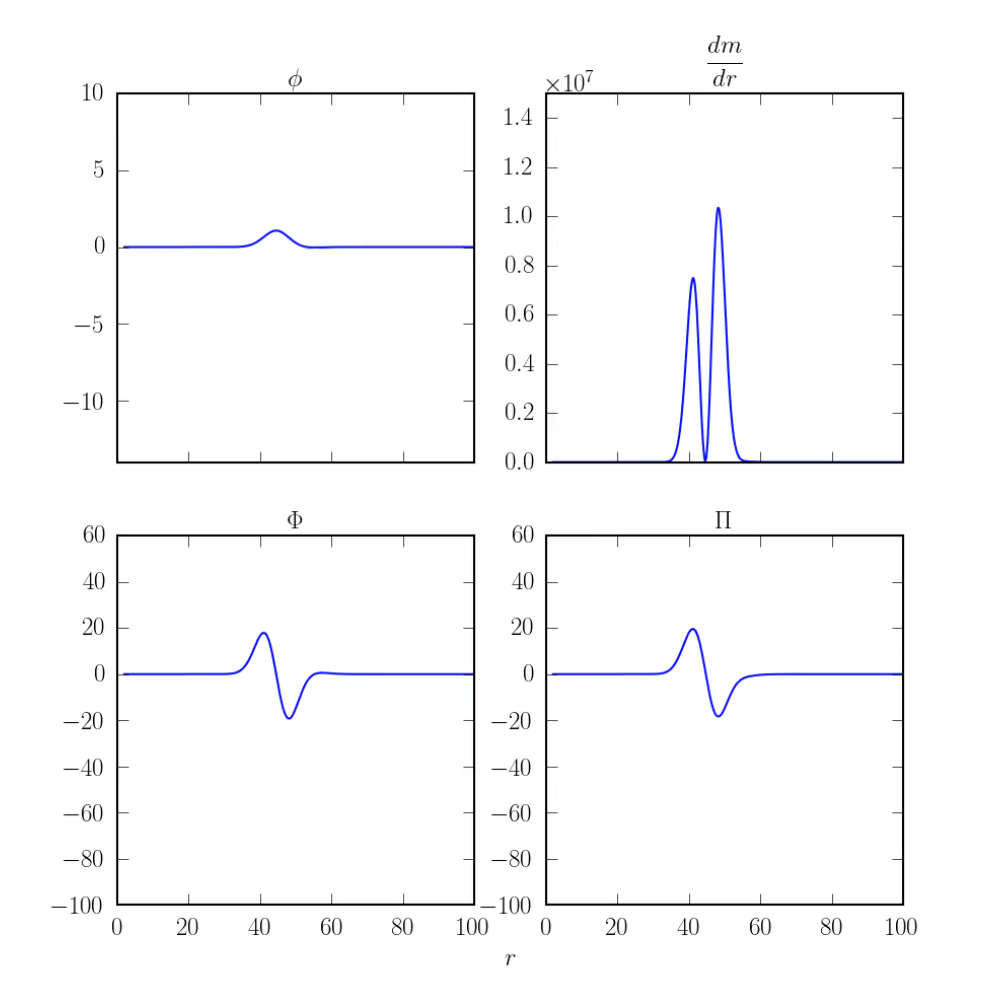
\includegraphics[width=0.75\textwidth]{video_output.png}
	\caption{Screenshot of the video output from the code for $\Delta = 5$.  It takes about 8 minutes for the code to produce this movie with preset resolution parameters.}
\end{figure}

\begin{figure}
	\centering
	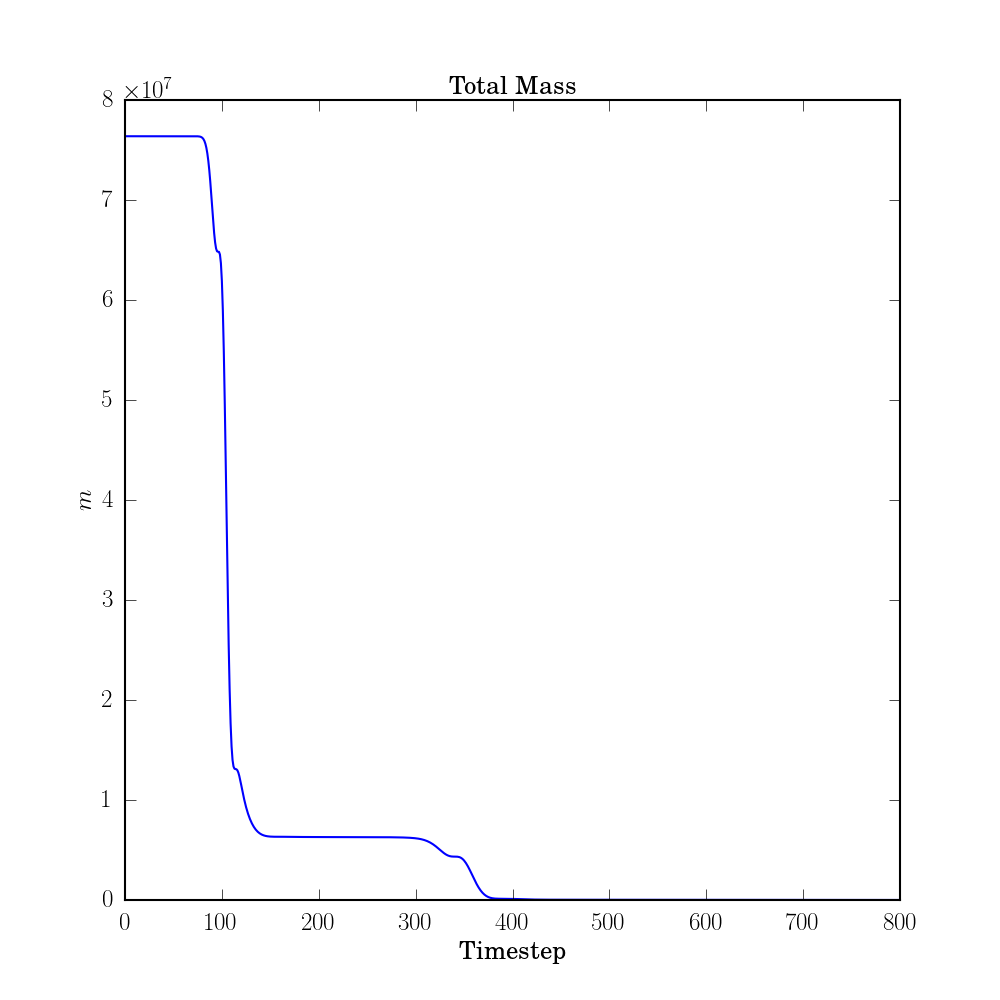
\includegraphics[width=0.75\textwidth]{total_mass_d5.png}
	\caption{Total mass plot, as produced by integrating the mass aspect function $\frac{d m}{d r}$ over the spatial window $r \in [2M, R]$.  Time progresses toward the right.  Note that in the beginning the total mass is constant as the pulse propagates toward the black hole, then suddenly decreases as some of the pulse is absorbed.  The amount that is reflected from the hole then propagates outward, and the total mass drops to nearly zero as the reflected pulse leaves the spatial window.}
\end{figure} 

Finally, the project outline asks us to determine how the width of the pulse $\Delta$ affects the amount of scalar radiation absorbed by the black hole.  The amount of absorbed radiation may be read off of the total mass plot (see figure 2), and the summary of this data from a few runs of the code is shown in figure 3, below.
\begin{figure}[h!]
	\centering
	\begin{tabular}{ l | c }
		$\Delta$ & Percent of Pulse Absorbed  \\
		\hline
		\hline
		5  & 90\% \\
		10 & 65\% \\
		15 & 40\% \\
		20 & 30\%
	\end{tabular}
	\caption{Table showing percent of pulse absorbed for a given value of the width of the Gaussian pulse, $\Delta$.}
\end{figure}
	


\end{document}